\documentclass{beamer}
\usetheme{Boadilla}

\usepackage{beamerthemesplit}
\usepackage[latin2]{inputenc}
\usepackage{colortbl}
\usepackage{hhline}
\usepackage{ae,aecompl,amsfonts}
\usepackage{fancyhdr}
\usepackage{hyperref}
\usepackage{verbatim}
\usepackage{array}
\usepackage{pstricks}
\usepackage{listings}
\usepackage{multirow}
\usepackage{wrapfig}
\usepackage{caption}
\usepackage{subcaption}

\captionsetup[subfigure]{labelformat=empty}

\def\hilite<#1>{%
\temporal<#1>{\color{gray}}{\color{blue}}%
{\color{blue!25}}}


\title[Recent \& Relevant experience]{Background in Web Development}
\author{Micha� Nowotka  \\  \small{job applicant}}
\institute{
\includegraphics[width=0.25\textwidth]{images/Chembl} \\  EMBL-EBI \\   ChEMBL group}
\date{\today}

  \begin{document}

	\frame{\titlepage}

	\frame
	{
		\tableofcontents
	}

    \section{Experience in research}

      \subsection{Bachelor tesis}

	\frame[plain]
	{
		\frametitle{The problem of haplotype frequency estimation -- bacelor thesis}

		\begin{wrapfigure}{l}{0.43\textwidth}
			\centering
			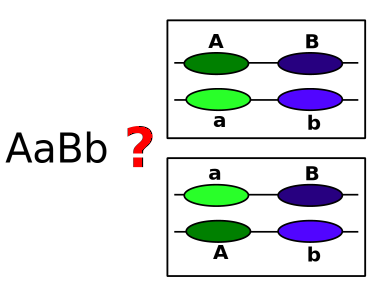
\includegraphics[width=0.43\textwidth]{images/poli}
			\caption{\small{Inferring haplotypes from genotypes}}
		\end{wrapfigure}
		$\bullet$~Determining~haplotypes~with~laboratory methods~is~expensive~and time-consuming. \\ \medskip
		$\bullet$~In~contrast,~there~are~many~cost-effective~techniques~for~determining genotypes. \\ \medskip
		$\bullet$~In general, it could be impossible to inferre haplotypes from genotype data.

		\begin{figure}
			\begin{center}
				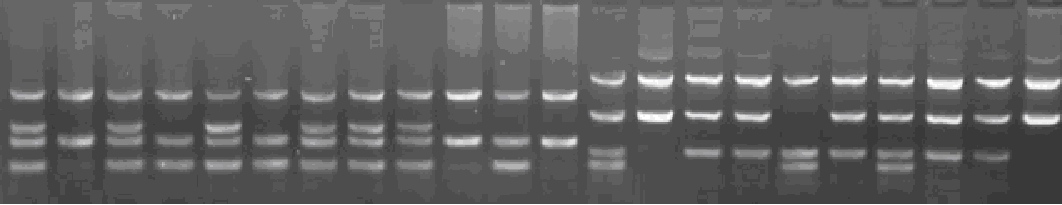
\includegraphics[width=\textwidth]{images/polimorfizmKIR}
				\caption{\small{Determining~genotype~experiment~results}}
			\end{center}
		\end{figure}
	}

	\frame[plain]
	{
		\frametitle{Idea of short overlapping windows}

		\begin{block}{Problem}
			Every algorithm emploing full space search would operate with $O(c^{n})$ complexity.
			This is why it cannot be directly applied to phasing long genotypes.
		\end{block}

		\begin{block}{Solution -- Genotypes can be divided into shorter pieces that overlap.}
			\begin{itemize}
				\item Piece length is fixed, so is computation time.
				\item Phasing n pieces has now $O(n)$ complexity.
				\item Multiple pieces can be phased in parrallel.
				\item If phasing algorithm is convergent total error should not be large.
			\end{itemize}
		\end{block}

		\begin{figure}
			\begin{center}
				
\includegraphics[width=0.40\textwidth]{images/window}
				\caption{\small{What are the error and execution time as a function of \textbf{width} i \textbf{overlap} parameters?}}
			\end{center}
		\end{figure}
	}

	\frame
	{

		\frametitle{Results}

		\begin{figure}
			\begin{subfigure}[b]{0.5\textwidth}
				\centering
				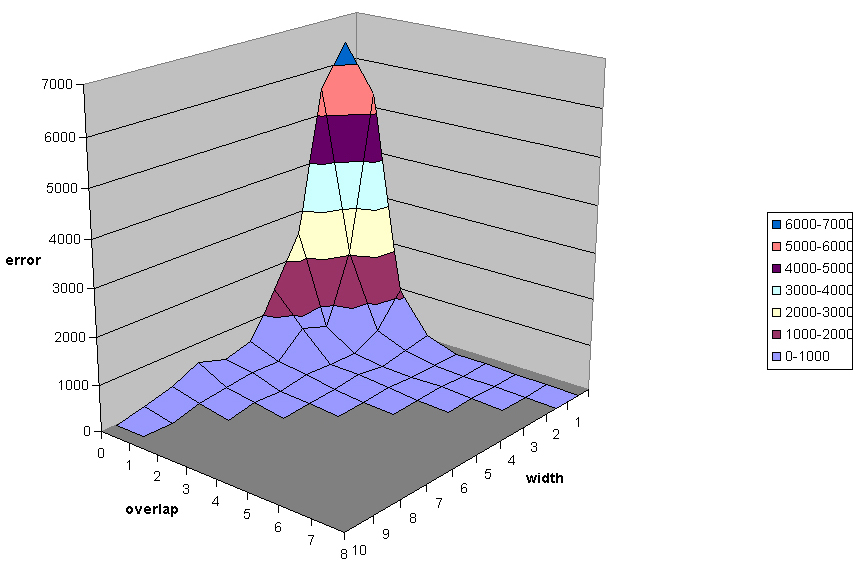
\includegraphics[width=\textwidth]{images/error}
				\caption{Error as a function of with and overlap parameters}
				\label{fig:error}
			\end{subfigure}%
			~
			\begin{subfigure}[b]{0.5\textwidth}
				\centering
				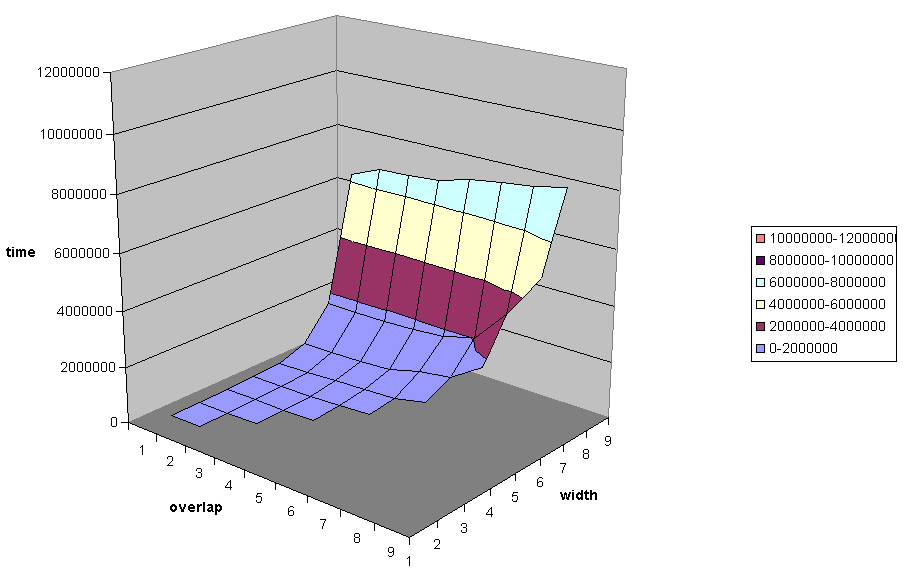
\includegraphics[width=\textwidth]{images/czas}
				\caption{Execution time as a function of with and overlap parameters}
				\label{fig:time}
			\end{subfigure}
		\end{figure}
	}

	\frame[plain]
	{
		\frametitle{Application architecture}

		\begin{center}
			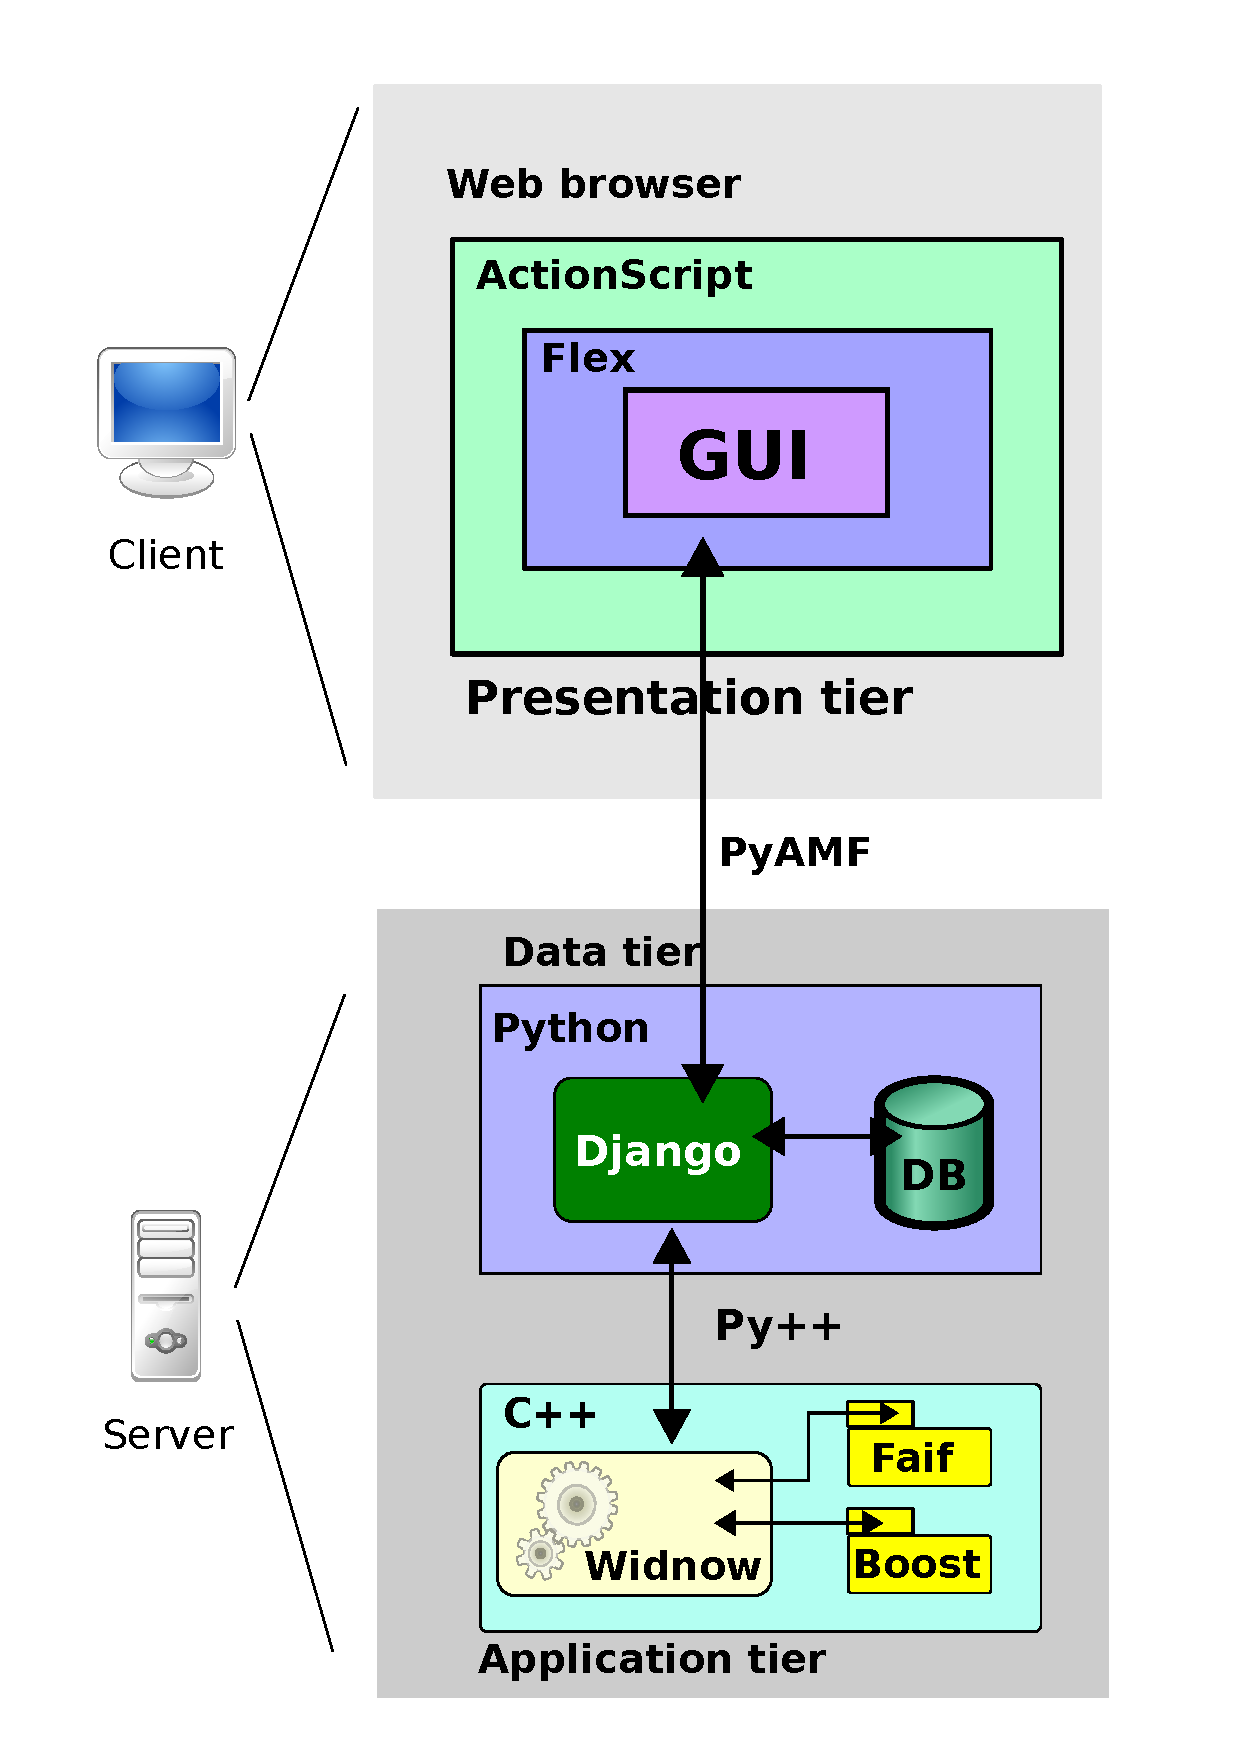
\includegraphics[width=0.47\textwidth]{images/scheme}
		\end{center}
	}

      \subsection{Master tesis}

	\frame[plain]
	{
		\frametitle{Automated functional annotation using classification algorithms and data fusion -- master thesis}

		\begin{block}{Functional genomics as a major field in applied bioinformatics}
			\begin{itemize}
				\item Functional interpretation is a key step in the analysis of DNA and protein sequences.
				\item This task cannot be done without availability of extensive functional annotation of the datasets.
				\item Due to the fast development of high-throughput sequencing technologies, an increasing amount of novel, uncharacterized sequence data have arisen.
				\item Stabdarized functional annotation is essential.
			\end{itemize}
		\end{block}
				
		\begin{block}{The goal}
			Privide biologists useful informartion to take into account when addressing the task of functionally characterizing thei requence data.
		\end{block}
	}

	\frame
	{
		\frametitle{Automated functional annotation -- the algorithm}

		\begin{block}{Input}
			Uncharacterized DNA or protein sequence.
		\end{block}

		\begin{itemize}
			\item BLAST.
			\item Gene Ontology lookup.
			\item Data fusion and inferrence.
		\end{itemize}
				
		\begin{block}{Output}
			Inferred functional annotation for the input sequence
		\end{block}
	}

	\frame
	{
		\frametitle{Inferring functional annotation}
				
		\begin{block}{For combining multiple results the Dempster's rule of combination is used.}

			\begin{itemize}
				\item Often used as a method of sensor fusion.
				\item Strongly emphasises the agreement between multiple sources and ignores all the conflicting evidence.
				\item Better alternative to weighted voting.
			\end{itemize}

		\end{block}
	}

	\frame[plain]
	{
		\frametitle{Application architecture}

		\begin{center}
			\includegraphics[width=0.47\textwidth]{images/scheme1}
		\end{center}
	}

    \section{Experience at CERN}

	\frame
	{
		\frametitle{Site Status Board -- an application monitoring the behavior of all the centers of a particular VO}
			  
		\begin{itemize}
			\item SSB provides a single entry point that summarizes the status of the sites.
			\item The main idea is to provide a flexible framework which would allow VOs to define multiple monitoring metrics.
			\item The metrics can be added, deleted and easily modified.
			\item The most critical metrics can be combined into a single value for each site corresponding to its status.
			\item SSB keeps the history of how all the metrics have evolved over time..
			\item SSB consists of three components: collectors that gather information, a database and a web server.
		\end{itemize}					  		
	}

	\frame
	{
		\frametitle{SSB -- implemented features}
			  
		\begin{itemize}
			\item XSLT replaced by Java Script template system.
			\item New coherent GUI.
			\item Filtering, paging, sorting in Expanded Table, computed on server side.
			\item Expanded Table ready for large amount of data.
			\item Redesigned backend.
			\item Client-side plotting.
			\item Bookmarking, undo/redo.
			\item Backbone.
		\end{itemize}					  		
	}

	\frame
	{
		\frametitle{Old and new SSB}

		\begin{figure}[h!]
			\centering
			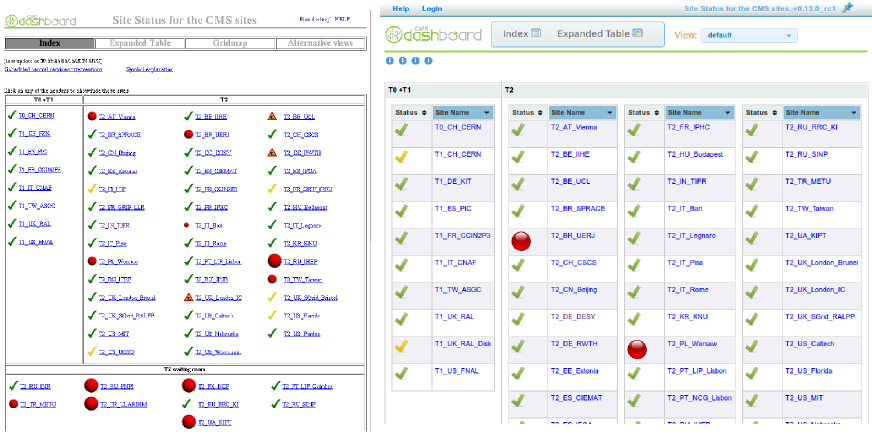
\includegraphics[width=1.0\textwidth]{images/chome}
		\end{figure}						  		
	}	

	\frame
	{
		\frametitle{Old and new SSB}

		\begin{figure}[h!]
			\centering
			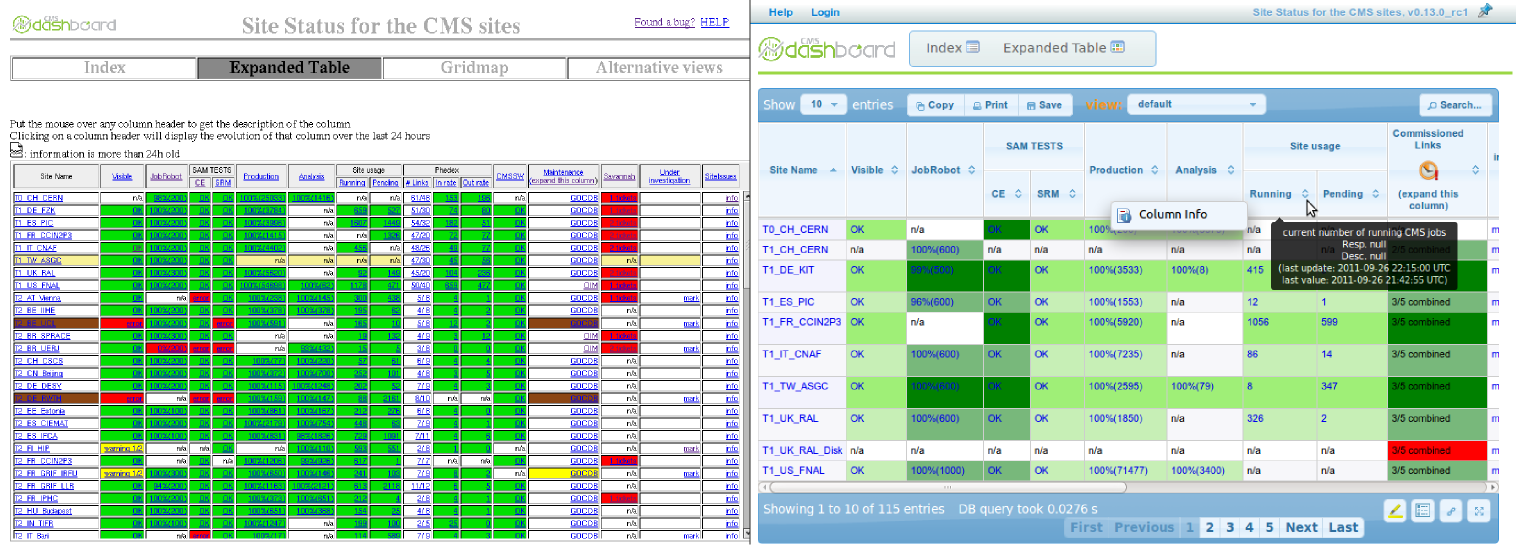
\includegraphics[width=1.0\textwidth]{images/ctable}
		\end{figure}						  		
	}
			
	\frame
	{

		\frametitle{Old and new SSB}

		\begin{figure}[h!]
			\centering
			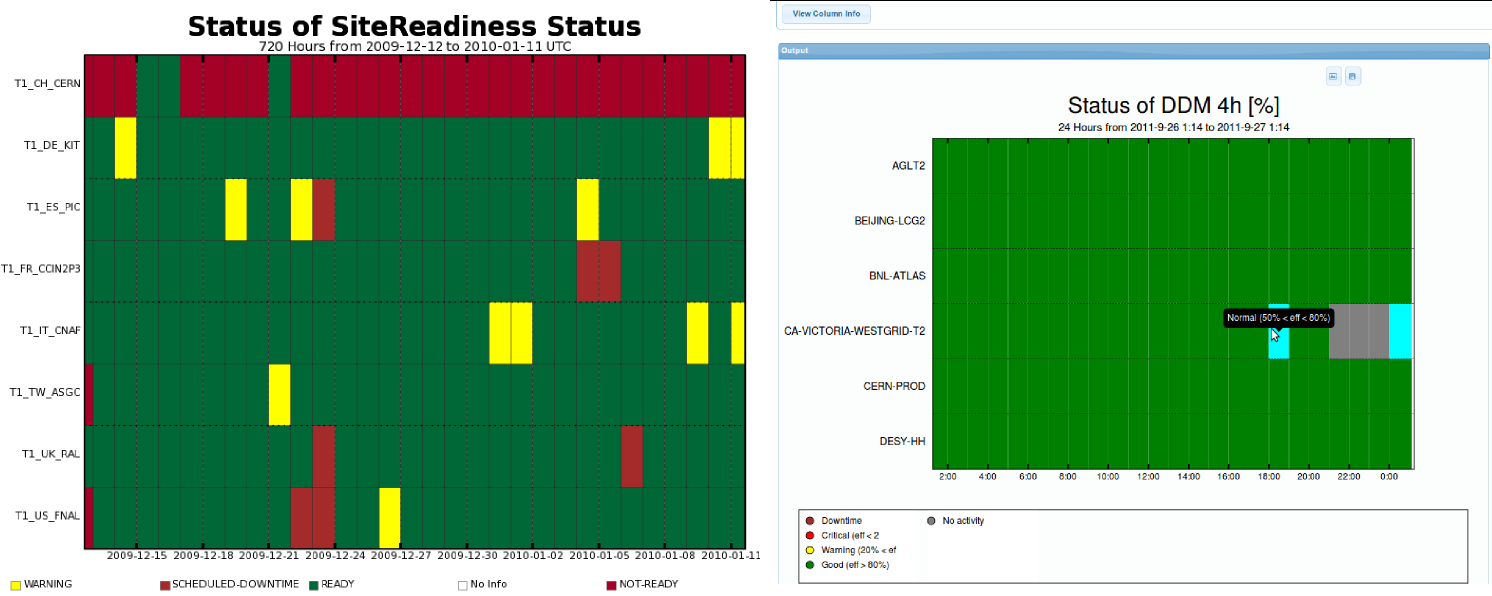
\includegraphics[width=1.0\textwidth]{images/chistory}
		\end{figure}						  		
	}
	
	\frame
	{
		\frametitle{SSB -- collector metainformation}
			  
		\begin{figure}[h!]
			\centering
			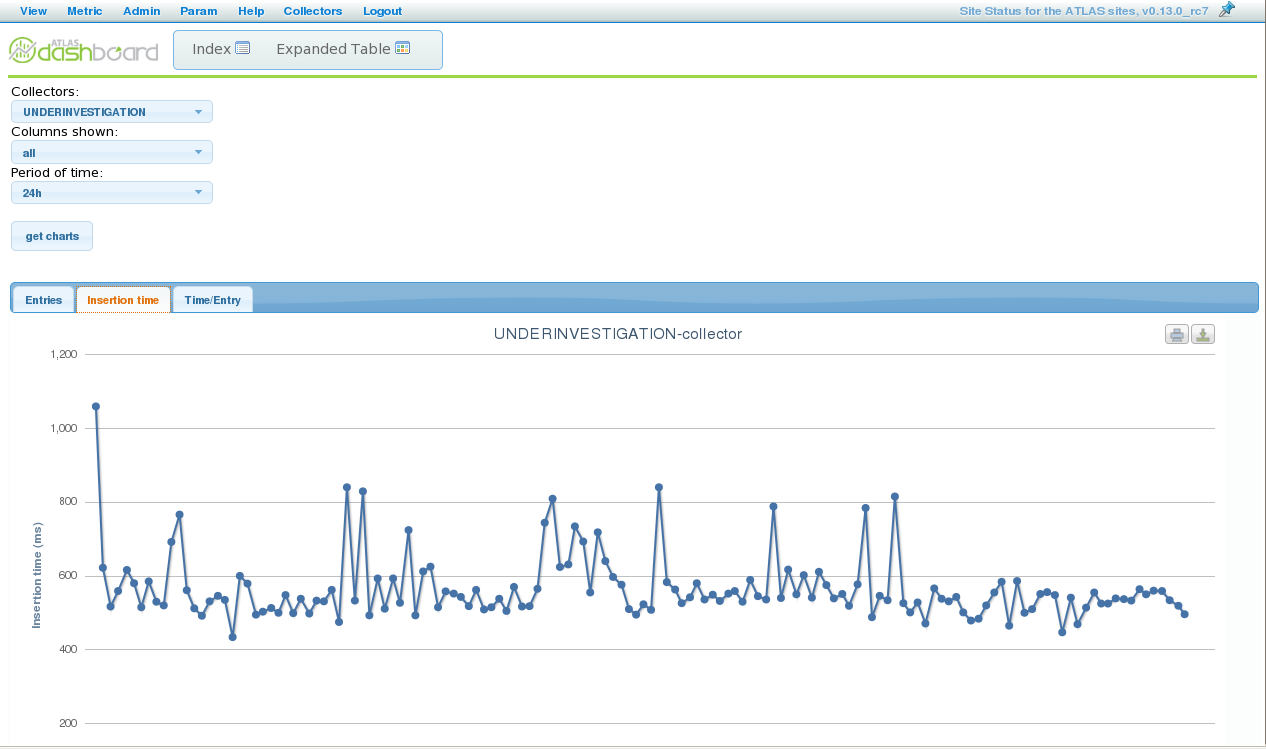
\includegraphics[width=1.0\textwidth]{images/meta}
		\end{figure}					  		
	}
		
	\frame
	{
		\frametitle{SSB -- TODO}
			  
		\begin{itemize}
			\item Tests (jQunit, Selenium).
			\item Database synchronization.
			\item Web based installation wizard.
			\item Getting rid of FOUCs.
			\item Refactoring of DAO.
			\item Expanded Table should refresh periodically and highlight recent changes.
			\item NoSQL for Sieview Data.
		\end{itemize}				  		
	}
			
	\frame
	{

		\frametitle{SSB -- Impact chart}

		\begin{figure}[h!]
			\centering
			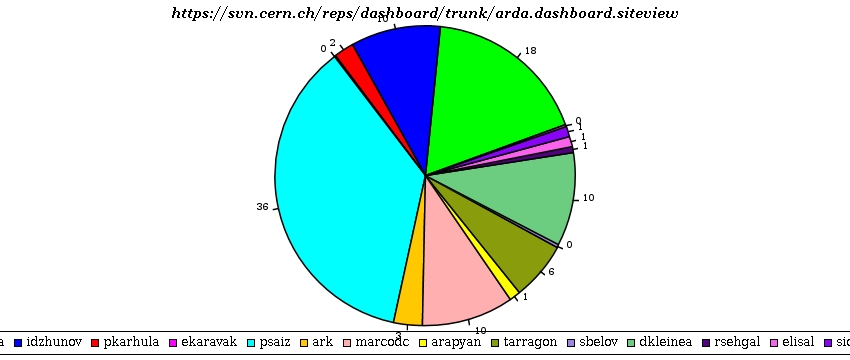
\includegraphics[width=1.0\textwidth]{images/percent}
		\end{figure}						  		
	}
			
	\frame
	{

		\frametitle{SSB -- Commits}

		\begin{figure}[h!]
			\centering
			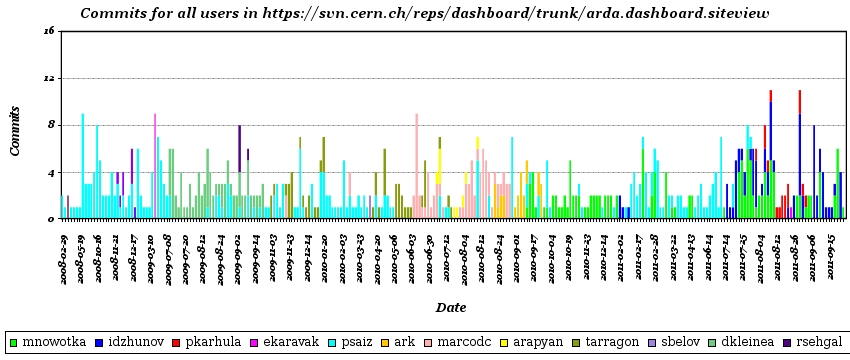
\includegraphics[width=1.0\textwidth]{images/all}
		\end{figure}						  		
	}
			
	\frame
	{

		\frametitle{SSB -- My commits}

		\begin{figure}[h!]
			\centering
			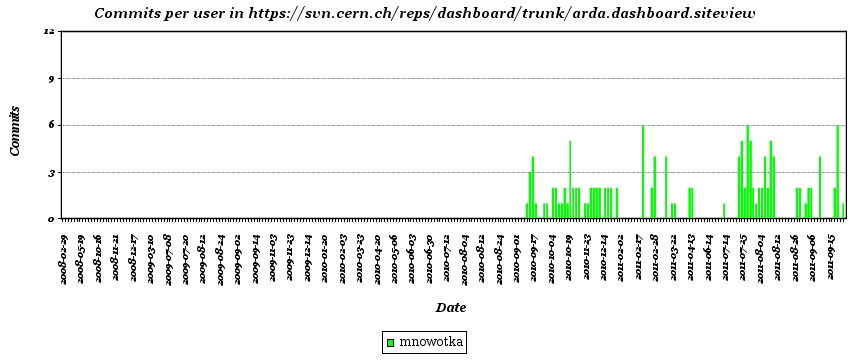
\includegraphics[width=1.0\textwidth]{images/commits}
		\end{figure}						  		
	}
			
	\frame
	{
		\frametitle{Framework}
			  
		\begin{block}{Benefits for the dashboard framework:}
			  
			\begin{itemize}
				\item Coherent set of tools and libraries.
				\item Proofs of concepts.
				\item Authentication mechinsms implemented in framework.
				\item Better documentation.
			\end{itemize}

		\end{block}
	}

	\frame
	{
		\frametitle{MonAlisa}
			  
		\begin{itemize}
			\item Installation on every node.
			\item Instalation and tuning of ML Repository.
			\item Alarms.
			\item New Metrics.
		\end{itemize}					
	}
			
	\frame
	{
		\frametitle{MonAlisa}
			  
		\begin{figure}[h!]
			\centering
			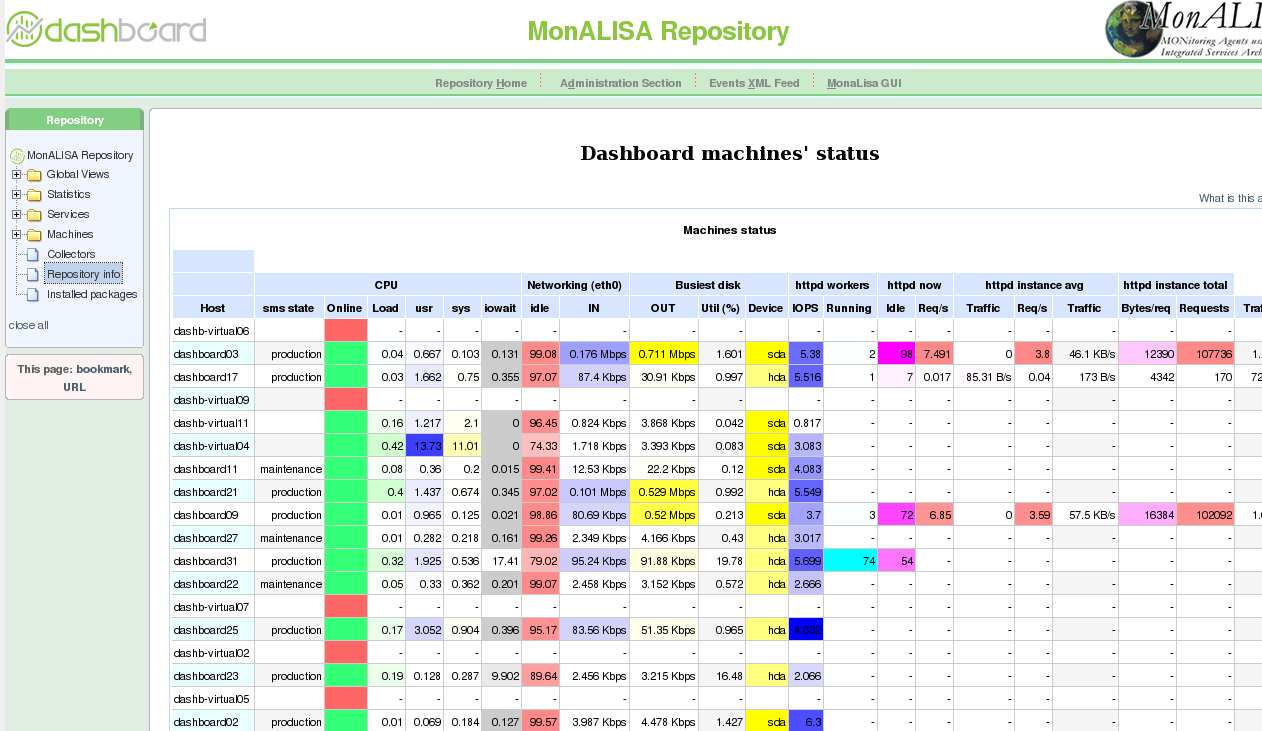
\includegraphics[width=1.0\textwidth]{images/monalisa}
		\end{figure}		
	}
			
	\frame
	{
		\frametitle{Other applications}
			  
		\begin{itemize}
			\item Dashboard for Google Eearth.
			\item SiteView.
		\end{itemize}
	}
	
	\frame
	{
		\frametitle{Peresentations}
			  
		Group meetings presentation:
			  
		\begin{itemize}
			\item jQuery.
			\item Charting.
			\item Deployment and load balancing.
			\item noSQL.
			\item Architecture of JS applications.
		\end{itemize}
	}
			
	\frame[plain]
	{
		\frametitle{Twiki}
			  
		Twiki articles:
			  
		\begin{itemize}
			\item JS tools and libraries (\url{https://twiki.cern.ch/twiki/bin/view/ArdaGrid/Libs}).
			\item MVC architecture (\url{https://twiki.cern.ch/twiki/bin/view/ArdaGrid/ModelViewController}).
			\item Dashboard services documentation (\url{https://twiki.cern.ch/twiki/bin/view/ArdaGrid/Services}).
			\item MonAlisa installation procedure (\url{https://twiki.cern.ch/twiki/bin/view/ArdaGrid/MonAlisa}).
			\item Authentication mechanism in dashboard framework (\url{https://twiki.cern.ch/twiki/bin/view/ArdaGrid/Auth}).
			\item Form handling (\url{https://twiki.cern.ch/twiki/bin/view/ArdaGrid/FormHandling}).
			\item Google Earth emergency (\url{https://twiki.cern.ch/twiki/bin/view/ArdaGrid/DashbEarth}).
		\end{itemize}						  		
	}
			
	\frame
	{
		\frametitle{Other}
			  
		\begin{itemize}
			\item Contributing to CHEP papers.
			\item Attending to Daily Ops.
			\item Attending to CMS Ops.
			\item Summer Student.
		\end{itemize}						  		
	}			
	
	\frame
	{
		\frametitle{What I learned}
			  
		\begin{itemize}
			\item Java Script technologies.
			\item Dashboard Framework.
			\item CERN School of Computing.
			\item Sys Admin stuff.
			\item Many interesting lectures (including Richard Stallman and James Watson).
			\item French course.
			\item Working in multinationa environment.
			\item Working in large organisation.
			\item Living abroad.
			\item Faster than light neutrino.
		\end{itemize}						  		
	}

    \section{Recent experience and current work}

	\frame
	{
		\frametitle{Horus.pl}

		\begin{figure}
			\begin{center}
				
\includegraphics[width=0.15\textwidth]{images/logo-horus}
			\end{center}
		\end{figure}

		Development of business applications intended to use by corporate clients:

		\begin{figure}
			\begin{subfigure}[b]{0.22\textwidth}
				\centering
				
\includegraphics[width=0.25\textwidth]{images/orange}
				\caption{Orange}
			\end{subfigure}%
			~
			\begin{subfigure}[b]{0.22\textwidth}
				\centering
				
\includegraphics[width=0.25\textwidth]{images/t-mobile}
				\caption{T-mobile}
			\end{subfigure}
			~
			\begin{subfigure}[b]{0.22\textwidth}
				\centering
				
\includegraphics[width=0.50\textwidth]{images/play}
				\caption{Play}
			\end{subfigure}
			~
			\begin{subfigure}[b]{0.22\textwidth}
				\centering
				
\includegraphics[width=0.35\textwidth]{images/netia}
				\caption{Netia}
			\end{subfigure}
		\end{figure}						  		
	}

	\frame
	{
		\frametitle{Horus Workflow}
			  
		\begin{block}{Horus Workflow} 
			Horus Workflow is used to define and monitor workflow in business processes. 
			It supports the implementation of any number of administrative processes, personnel, management or sales. 
		\end{block}


		Horus Workflow System Features:

			  
		\begin{itemize}
			\item Support for managing tasks
			\item The ability to define own processes
			\item Support for document management processes
			\item Support for a variety of organizational structures
			\item Monitoring of user activity (change history)
			\item Management of the company organizational structure
		\end{itemize}
	}  			

	\frame
	{

		\frametitle{Horus Workflow -- application screenshot}

		\begin{figure}[h!]
			\centering
			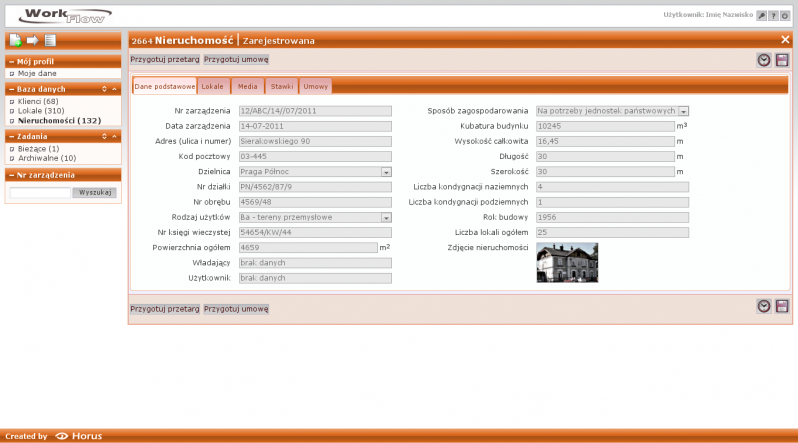
\includegraphics[width=.75\textwidth]{images/workflow}
		\end{figure}						  		
	}

	\frame
	{
		\frametitle{Horus Workflow -- technologies}
			  
		Used technologies and libraries:
			  
		\begin{itemize}
			\item Spring
			\item Maven
			\item JBoss
			\item Hudson / Jenkins
			\item Coffee Script
			\item JQuery UI
		\end{itemize}
	}

	\frame
	{
		\frametitle{TMS Brokers Brokerage House}

		
\includegraphics[width=0.18\textwidth]{images/tms}				 

		\begin{block}{Tasks and responsibilities:}

			\begin{itemize}
				\item Development of financial reporting software
				\item Supporting promotional campaigns
				\item MetaTrader API programming
			\end{itemize}

		\end{block}
	}

	\frame
	{
		\frametitle{TMS Brokers -- technologies}
			  
		Used technologies and libraries:

			  
		\begin{itemize}
			\item JQuery UI
			\item Highcharts and Highstock
			\item Python
			\item Django
			\item C++
		\end{itemize}
	}    

	\frame
	{
		\begin{figure}[h!]
			\centering
			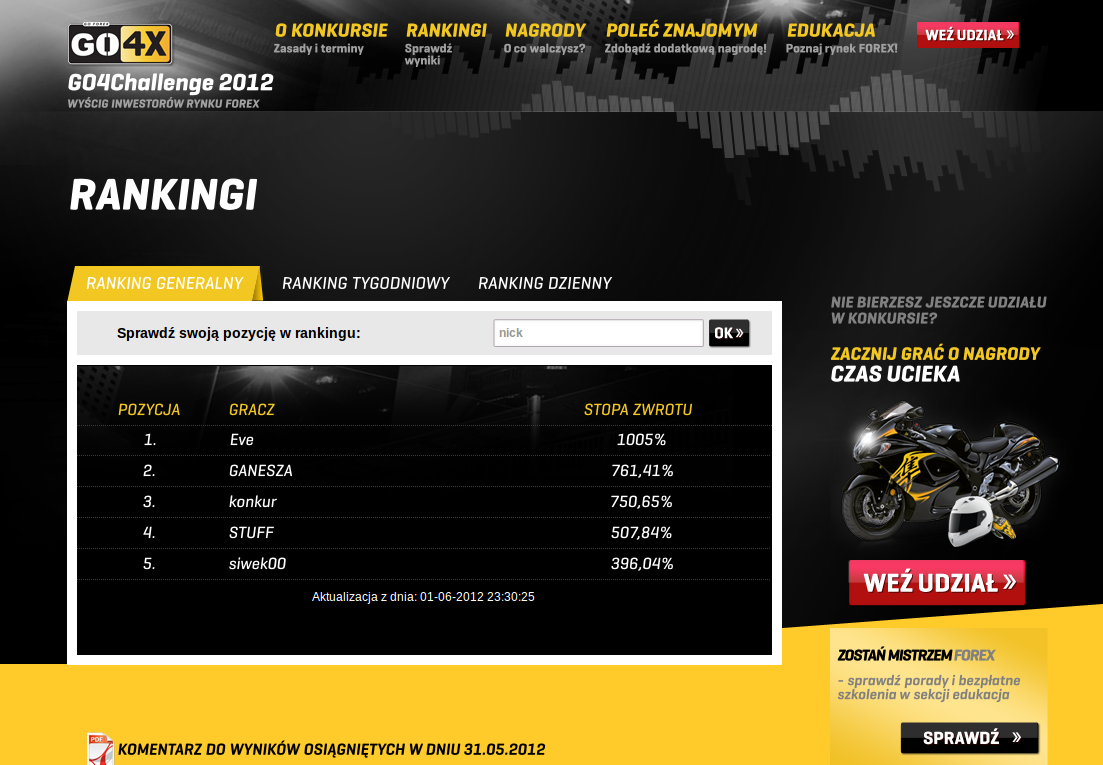
\includegraphics[width=0.9\textwidth]{images/challange}
		\end{figure}						  		
	}

	\frame
	{
		\frametitle{Github}

		\begin{block}{Source}

			\LaTeX~source of this presentation can be downloaded from github:

			\begin{center}
				\texttt{git://github.com/mnowotka/Chembl-job-web.git}
			\end{center} 
		\end{block}					  		
	}
			
	\frame
	{
		\begin{center}
			\huge{\textbf{\textit{Thank you for your attention.}}}
		\end{center} 
	}

\end{document}
